\documentclass[11pt,reqno]{amsart}
%==============================================================
%  Transport and tiling bounds for the affine plank problem on the triangle:
%  new sharp cases, a rigidity theorem, and a normalizer obstruction.
%
%  ACADEMIC-CORRECTNESS POLICY (binding): every Theorem/Proposition/Lemma is
%  either cited (with attribution) or proved in full here. Not-yet-established
%  statements live in Conjecture/Problem/Remark and are never used as proved.
%  SCOPE (honest): this studies the triangle as a CONCRETE body plus method.
%  It is NOT an attack on the general conjecture via Ambrus (whose reduction
%  targets simplices of dimension 2N-1; the triangle is never a target).
%==============================================================
\usepackage{amsmath,amssymb,amsthm,mathtools}
\usepackage{tikz}
\usepackage[margin=1.1in]{geometry}
\usepackage[colorlinks=true,linkcolor=blue,citecolor=blue]{hyperref}
\theoremstyle{plain}
\newtheorem{theorem}{Theorem}[section]
\newtheorem{proposition}[theorem]{Proposition}
\newtheorem{lemma}[theorem]{Lemma}
\newtheorem{corollary}[theorem]{Corollary}
\theoremstyle{definition}
\newtheorem{conjecture}[theorem]{Conjecture}
\newtheorem{definition}[theorem]{Definition}
\newtheorem*{pocketlemma}{Pocket Lemma}
\newtheorem{problem}[theorem]{Problem}
\theoremstyle{remark}
\newtheorem{remark}[theorem]{Remark}
\newcommand{\rw}{\operatorname{rw}}
\newcommand{\Leb}{\operatorname{Leb}}
\newcommand{\R}{\mathbb{R}}
\DeclareMathOperator{\wid}{w}
\DeclareMathOperator{\vol}{vol}

\title{Transport and tiling bounds for the affine plank problem on the triangle}
% AUTHOR BLOCK — decision pending (see 03-work-plan.md §5); fill before submission.
\author{[Author names]}
\address{[Affiliation]}
\email{[email]}
\subjclass[2020]{52C17 (52A40, 52A10)}
\keywords{Plank problem, relative width, affine plank conjecture, covering,
rigidity, witness measure}
\date{Draft --- \today}

\begin{document}
\begin{abstract}
Bang's affine (relative-width) plank conjecture asserts that if a convex body $K$
is covered by planks $P_1,\dots,P_n$ then $\sum_i \rw_K(P_i)\ge 1$, where
$\rw_K(P)=\wid(P)/\wid_K(u_P)$ is the width of $P$ relative to the width of $K$ in
$P$'s direction. It is open for non-symmetric bodies, already in the plane. We
study the triangle, developing a \emph{transport} method (witness measures with
uniform marginals) alongside boundary tilings. Main results: (1) three planks
parallel to the medians satisfy $\sum\rw\ge1$, with equality if and only if each
is the central third of its median; (2) an explicit witness measure for every
cyclic triple whose mid-level lines concur (a two-parameter family), with the
bound attained at each member by a covering that is unique for its directions;
(3) a characterization: for three pairwise non-parallel directions on the
triangle, a witness measure exists if and only if the mid-level lines concur ---
settling the existence question of Gardner (1988) for three directions on the
triangle; (4) a quantification of the method off the concurrent locus by a
\emph{transport defect} $D(u)$, with $\sum\rw\ge1/D(u)$ for coverings by planks
parallel to the given triple: $D=\tfrac32$ exactly at the facet triple, and near
concurrence $D\le1+O(\varepsilon)$, so that planks parallel to any cyclic triple
with parameters within $\tfrac1{60}$ of the medians satisfy
$\sum\rw\ge\tfrac{27}{29}>4\sqrt3-6$ --- past the constant of
Bakaev--Yehudayoff on the triangle, but only for these restricted direction
families, whereas their bound is uniform over all coverings; (5) on the
$3$-simplex, a one-parameter family of concurrent direction quadruples carrying
explicit skeleton witness measures. Supporting results: $\sum\rw\ge1/d$ for
$d\ge2$ via the uniform measure, sharp two-direction and facet-parallel cases,
the ``three facets $+$ one plank'' case, and sharpness of the chord-lemma step
in Bang's sign argument. All our theorems bound coverings by planks in specified
direction families on a fixed body, or characterize witness measures; none
resolves the conjecture for the triangle, let alone the plane.
\end{abstract}
\maketitle

\section{Introduction}\label{sec:intro}

A \emph{plank} of width $w$ is the region between two parallel hyperplanes at
distance $w$. For a convex body $K\subset\R^d$ and a plank $P$ with unit normal $u$,
the \emph{relative width} of $P$ is $\rw_K(P)=\wid(P)/\wid_K(u)$, where
$\wid_K(u)=\max_{x\in K}\langle u,x\rangle-\min_{x\in K}\langle u,x\rangle$. Bang's
affine plank conjecture~\cite{Bang51,Ambrus} states:
\begin{conjecture}[Affine plank problem; Bang 1951]\label{conj:bang}
If $K$ is covered by planks $P_1,\dots,P_n$, then $\sum_{i=1}^n \rw_K(P_i)\ge 1$.
\end{conjecture}
Ball~\cite{Ball91} proved Conjecture~\ref{conj:bang} for centrally symmetric $K$.
For general bodies it is open, and, as emphasised by Bakaev--Yehudayoff~\cite{BY26},
it is open \emph{already in the plane} --- only the two-plank case is settled there.
The best general lower bound is
$\sum\rw\ge 2/(1+\sqrt d)$~\cite{BY26}; on the equilateral triangle their method
gives $\sum\rw\ge 4\sqrt3-6\approx0.928$.

\smallskip
\noindent\textbf{Scope.}\ This paper studies the triangle as a concrete body and
develops the associated \emph{transport} (witness-measure) and \emph{tiling}
methods. It is \emph{not} an attack on Conjecture~\ref{conj:bang} through the Ambrus
reduction: that reduction sends a covering by $N$ planks to a simplex of dimension
$2N-1$, so the triangle (the $2$-simplex) is never a target
(Remark~\ref{rem:ambrus}). Our results are new sharp cases for a fixed body, a
rigidity theorem, a dimension-agnostic structural characterization, and an
obstruction; we prove nothing about the general conjecture. Since the
distinctions matter, we spell them out: five statements should be kept apart ---
(a) bounds for coverings by planks parallel to a \emph{fixed direction family};
(b) existence and characterization of \emph{witness measures}; (c) bounds for
\emph{all} coverings of the triangle; (d) Conjecture~\ref{conj:bang} for the
triangle; (e) Conjecture~\ref{conj:bang} in the plane. Every theorem in this
paper lives at level (a) or (b); at level (c) we prove nothing beyond the
universal $1/d$ of Theorem~\ref{thm:oned}, and (d), (e) remain wide open.

\begin{remark}\label{rem:ambrus}
Ambrus's reduction~\cite{Ambrus} sends a covering by $N$ planks to a covering of a
simplex of dimension $2N-1$ (two points per plank). The target simplices thus have
odd dimension growing with $N$; the $2$-simplex (triangle) is never among them. So
proving the conjecture for the triangle does \emph{not} imply the planar case, and
our results are about the triangle as a concrete body, not a reduction of
Conjecture~\ref{conj:bang}.
\end{remark}

\subsection*{The triangle model}
By affine invariance take $\Delta=\{x\in\R^3:x_i\ge0,\ x_1+x_2+x_3=1\}$. A
normalized plank is $P=\{x\in\Delta: f(x)\in I\}$ with $f:\Delta\to[0,1]$ affine
onto $[0,1]$ and $I\subset[0,1]$ an interval; then $\rw_\Delta(P)=|I|$. Covering
means $\Delta\subset\bigcup_i P_i$. The restriction $I\subset[0,1]$ loses no
generality: replacing $I$ by $I\cap[0,1]$ leaves $P\cap\Delta$ unchanged and does
not increase $|I|$.

\subsection*{Results}
Theorem~\ref{thm:oned} (\S\ref{sec:measure}), Theorems~\ref{thm:twodir}
and~\ref{thm:facet} (\S\ref{sec:sharp}), Theorem~\ref{thm:3plus1}
(\S\ref{sec:3plus1}), and the main results: Theorem~\ref{thm:median} with rigidity
(\S\ref{sec:median}); the weighted-perimeter Theorem~\ref{thm:wper}
(\S\ref{sec:concur}), which extends the sharp bound from the medians to a
two-parameter family of concurrent triples; and
Theorem~\ref{thm:tight}, which shows the bound is attained at every member of
that family by an explicit unique tight covering.
Proposition~\ref{prop:concur} (\S\ref{sec:concur}) is the dimension-agnostic
necessary condition, Corollary~\ref{cor:iff} the resulting characterization for
cyclic triples, and Theorem~\ref{thm:char} the full three-direction
characterization on the triangle. Section~\ref{sec:defect} quantifies the
method off the concurrent locus (the transport defect: exact value $\tfrac32$
at the facets, Theorem~\ref{thm:facetdefect}; linear stability near
concurrence, Theorem~\ref{thm:defectstab}; Corollary~\ref{cor:beyond} then
gives $\sum\rw\ge\tfrac{27}{29}>4\sqrt3-6$ near the medians --- for coverings
in the given direction families only, see Remark~\ref{rem:beyond});
\S\ref{sec:simplex3} constructs the witness family
on $\Delta^3$ (Theorem~\ref{thm:simplex3}). Proposition~\ref{thm:nogo} and
Remark~\ref{rem:nogo} (\S\ref{sec:nogo})
record the normalizer obstruction. Appendix~\ref{app:tilings} classifies the
boundary tilings of cyclic triples (Proposition~\ref{prop:tilings}), the
combinatorial engine behind both rigidity results.

\section{The uniform-measure bound $\sum\rw\ge 1/d$}\label{sec:measure}
\begin{theorem}\label{thm:oned}
Let $d\ge2$. If $K\subset\R^d$ is covered by planks $P_1,\dots,P_n$, then
$\sum_i\rw_K(P_i)\ge 1/d$. The per-plank estimate $\mu(P)\le d\,\rw_K(P)$ for the
uniform measure $\mu$ is sharp at the simplex; hence the argument, run with the
uniform measure, cannot improve the constant $1/d$. (For $d=1$ the conjecture
itself is trivial: intervals covering an interval satisfy $\sum\rw\ge1$.)
\end{theorem}
\begin{proof}
Let $\mu$ be the uniform probability measure on $K$. Fix $u$, normalize
$\langle u,\cdot\rangle\in[0,w]$, $w=\wid_K(u)$. The marginal density is
$f(t)=V(t)/\vol(K)$ with $V(t)=\vol_{d-1}(K\cap\{\langle u,\cdot\rangle=t\})$; by
Brunn--Minkowski $g:=V^{1/(d-1)}$ is concave on $[0,w]$. If $g$ peaks at $t^\ast$
with value $g^\ast$, then $g\ge g^\ast h$ for the tent $h$ ($h(0)=h(w)=0$,
$h(t^\ast)=1$), so $f=g^{d-1}\ge(\max f)\,h^{d-1}$ and
$1=\int f\ge(\max f)\int_0^w h^{d-1}=(\max f)\,w/d$, giving $\max f\le d/w$. Hence
$\mu(P)=\int_I f\le d\,\rw_K(P)$ for each plank, and
$1=\mu(K)\le\sum_i\mu(P_i)\le d\sum_i\rw_K(P_i)$. For sharpness of the per-plank
estimate: equality in $\max f\le d/w$ forces $V\propto h^{d-1}$ (conical sections),
realized by the simplex $K=\Delta^d$ with $u$ a vertex--facet direction, where a
thin plank at the facet has $\mu(P)=(d-o(1))\rw_K(P)$. Thus for the simplex the
\emph{uniform} measure cannot certify a constant larger than $1/d$ by the union
bound; this does \emph{not} assert any covering of the simplex with
$\sum\rw$ near $1/d$ (indeed Theorem~\ref{thm:facet} gives $\sum\rw\ge1$ for
facet-parallel coverings).
\end{proof}
\begin{remark}\label{rem:oneall}
Other measures do better for \emph{restricted} direction families: the witness
measures of \S\ref{sec:concur} certify the full constant $1$ for suitable triples,
and \S\ref{sec:defect} quantifies the best constant certifiable per triple. For
\emph{all} directions simultaneously, however, no single measure certifies the
constant $1$: uniform marginals in all directions would force
$\mathbb E[x_k]=\tfrac12$ against $\sum x_k=1$ (Gardner's
obstruction~\cite{Gardner88}). On the triangle the best constant certifiable by
one measure against all directions at once lies between $\tfrac12$ (the uniform
measure; Proposition~\ref{prop:defect}(iv)) and $\tfrac23$ (the facet triple
already forces it; Theorem~\ref{thm:facetdefect}); we do not pursue its exact
value.
\end{remark}

\section{Sharp cases: two directions and facet-parallel families}\label{sec:sharp}
\begin{theorem}\label{thm:twodir}
If every plank covering the triangle is parallel to one of two fixed
\emph{non-parallel} directions, then $\sum\rw\ge1$, and this is sharp. (If the two
directions are parallel the statement is trivial: all planks share one normalized
coordinate $f$, the intervals $f(P_i)$ cover $[0,1]$, and $\sum\rw=\sum|I_i|\ge1$.)
\end{theorem}
\begin{proof}
We use Gardner's existence theorem \cite[Theorem~1]{Gardner88}, whose exact
statement is: \emph{for a convex body $K\subset\R^n$ and two directions
$\theta_1,\theta_2$, there exists a relative-width measure on $K$ for
$\{\theta_1,\theta_2\}$} --- a probability measure $\nu$, possibly singular,
such that $\nu(S\cap K)$ equals the relative width of $S$ for every slab $S$
orthogonal to $\theta_1$ or $\theta_2$; equivalently, the pushforward of $\nu$
under each normalized affine coordinate $f_{\theta_i}:K\to[0,1]$ is
$\Leb[0,1]$. Applying this to $K=\Delta$ and our two directions gives $\nu$
with $f_{u\#}\nu=f_{v\#}\nu=\Leb$. Then $\nu(P)=|I|=\rw(P)$ for each plank, and
$1=\nu(\Delta)\le\sum\nu(P_i)=\sum\rw(P_i)$.
\end{proof}
\begin{theorem}\label{thm:facet}
Planks parallel to the facets of a simplex $\Delta^d$, in any number, that cover
$\Delta^d$ satisfy $\sum\rw\ge1$, and this is sharp.
\end{theorem}
\begin{proof}
Write $\Delta^d=\{\lambda\in[0,1]^{d+1}:\sum_k\lambda_k=1\}$ in barycentric
coordinates; a plank parallel to facet $k$ is a coordinate slab
$\{\lambda_k\in I\}$. Grouping the planks by facet, let
$U_k=\bigcup_{c(i)=k}I_i\subset[0,1]$ be the forbidden set on facet $k$, so
$\sum_k|U_k|\le\sum_i|I_i|=:R$, and set $C_k=[0,1]\setminus U_k$. A point
$\lambda\in\Delta^d$ is uncovered iff $\lambda_k\in C_k$ for every $k$; since
$C_k\subset[0,1]$, an uncovered point exists \emph{iff}
$1\in C_1+\dots+C_{d+1}$ (Minkowski sum).

Assume $R<1$; we produce an uncovered point. Each $U_k$ is a finite union of
closed intervals, so $C_k$ is a finite union of intervals, relatively open in
$[0,1]$, with $|C_k|=1-|U_k|\ge1-R>0$; it need not be compact, so fix
$\eta=\tfrac{1-R}{d+2}>0$ and choose a \emph{compact} $C_k'\subseteq C_k$ (shave
each component) with $|C_k'|\ge|C_k|-\eta$. The one-dimensional
Brunn--Minkowski inequality $|A+B|\ge|A|+|B|$ holds for nonempty compact
$A,B\subset\R$: $A+B\supseteq(A+\min B)\cup(\max A+B)$, and the two translates
meet only at $\max A+\min B$. Iterating it, $D:=C_1'+\dots+C_d'$ (compact)
satisfies $|D|\ge\sum_{k=1}^d|C_k'|\ge d-\sum_{k=1}^d(|U_k|+\eta)$; as
$D\subseteq[0,d]$,
$|[0,1]\setminus D|\le|[0,d]\setminus D|\le\sum_{k=1}^d(|U_k|+\eta)$, whence
$|D\cap[0,1]|\ge1-\sum_{k=1}^d(|U_k|+\eta)$. Also $(1-C_{d+1}')\cap[0,1]$ has
measure $|C_{d+1}'|\ge1-|U_{d+1}|-\eta$. Both sets lie in $[0,1]$ and their
measures sum to at least $2-R-(d+1)\eta>1$, so they intersect: there is $t\in D$
with $1-t\in C_{d+1}'$. Writing $t=\lambda_1+\dots+\lambda_d$ with
$\lambda_k\in C_k'\subseteq C_k$ and $\lambda_{d+1}=1-t\in C_{d+1}$ gives an
uncovered $\lambda\in\Delta^d$.
Contrapositively, covering forces $R\ge1$. Sharpness: the facet tiling
$I_k=[0,\tfrac1{d+1}]$ gives $\sum\rw=1$.
\end{proof}
\begin{remark}
The edge-by-edge argument does \emph{not} prove this: on an edge only two
barycentric coordinates vary, so no single edge can force $\sum_k|U_k|\ge1$ across
all $d+1$ facets. The Minkowski-sum reduction above is the correct route; note that
no witness \emph{measure} can prove it either, since facet directions violate the
concurrence condition of Proposition~\ref{prop:concur}.
\end{remark}

\section{Three facets plus one arbitrary plank}\label{sec:3plus1}
\begin{theorem}\label{thm:3plus1}
Let $P_i=\{\lambda_i\in I_i\}$ ($i=1,2,3$) be facet-parallel with $a_i=|I_i|$, and
let $Q=\{f\in J\}$, $t=|J|$, with $f:\Delta\to[0,1]$ affine normalized. If
$\Delta\subset P_1\cup P_2\cup P_3\cup Q$ then $a_1+a_2+a_3+t\ge1$.
\end{theorem}
\begin{proof}
Choose an active edge of $f$; relabelling, $f(v_j)=0$, $f(v_k)=1$, and let $v_i$ be
the opposite vertex, $\theta=f(v_i)$. For $s\in[0,1]$ consider the fibre
$F_s=\{\lambda_i=s\}$, parametrized by $u=\lambda_k\in[0,1-s]$, so
$\lambda_j=1-s-u$ and $f|_{F_s}(u)=\theta s+u$. On $F_s$: $P_i\cap F_s=F_s$ if
$s\in I_i$ (else $\varnothing$); $P_j\cap F_s$, $P_k\cap F_s$, $Q\cap F_s$ have
lengths $\le a_j,a_k,t$. Put $B=a_j+a_k+t$. If $s\notin I_i$ and $F_s$ is covered,
its length $1-s\le B$. If $B\ge1$ we are done; else $[0,1-B)\subset I_i$, so
$a_i\ge1-B$. In both cases $a_1+a_2+a_3+t=a_i+B\ge1$.
\end{proof}

\section{The median theorem and its rigidity}\label{sec:median}
Let $m_1,m_2,m_3$ be the medians of $\Delta$ as normalized affine forms: with
$A,B,C$ the vertices,
\[ m_1=(\tfrac12,0,1),\quad m_2=(0,1,\tfrac12),\quad m_3=(1,\tfrac12,0), \]
(vertex values). One has $m_1+m_2+m_3\equiv\tfrac32$. A \emph{median plank} is
$P_i=\{m_i\in I_i\}$, $I_i=[l_i,h_i]$, $r_i=|I_i|>0$.
\begin{theorem}\label{thm:median}
If three median planks cover $\Delta$, then $r_1+r_2+r_3\ge1$, with equality if and
only if $I_1=I_2=I_3=[\tfrac13,\tfrac23]$.
\end{theorem}
We are not aware of a previous tight \emph{non-facet} three-direction rigidity
result for the triangle: the sharp cases recorded in the survey
\cite{Verreault} (and in \cite{Gardner88,BY26}) concern facet/coordinate directions,
two directions, or symmetric bodies.

\begin{figure}[ht]
\centering
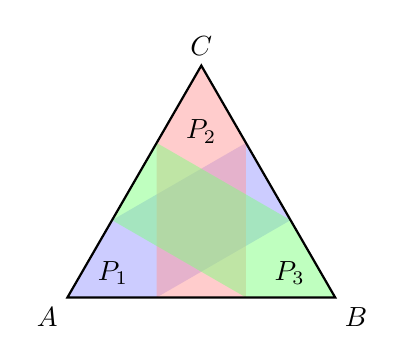
\begin{tikzpicture}[scale=3.4]
  \coordinate (A) at (0,0); \coordinate (B) at (1,0); \coordinate (C) at (0.5,0.866);
  \fill[blue!40,opacity=.5]  (0,0) -- (0.3333,0) -- (0.8333,0.2887)
       -- (0.6667,0.5773) -- (0.1667,0.2887) -- cycle;
  \fill[red!40,opacity=.5]   (0.3333,0) -- (0.6667,0) -- (0.6667,0.5773)
       -- (0.5,0.866) -- (0.3333,0.5773) -- cycle;
  \fill[green!50,opacity=.5] (0.6667,0) -- (1,0) -- (0.8333,0.2887)
       -- (0.3333,0.5773) -- (0.1667,0.2887) -- cycle;
  \draw[thick] (A) -- (B) -- (C) -- cycle;
  \node[below left]  at (A) {$A$};
  \node[below right] at (B) {$B$};
  \node[above]       at (C) {$C$};
  \node at (0.17,0.09)  {$P_1$};
  \node at (0.5,0.62)   {$P_2$};
  \node at (0.83,0.09)  {$P_3$};
\end{tikzpicture}
\caption{The tight median covering of Theorem~\ref{thm:median}:
$I_1=I_2=I_3=[\tfrac13,\tfrac23]$. Each plank $P_i=\{m_i\in[\tfrac13,\tfrac23]\}$
is the central-thirds band of its median; the three traces tile each edge, and
the planks cover $\Delta$ with $\sum\rw=1$.}
\label{fig:median}
\end{figure}
\begin{proof}[Proof of the bound]
Let $\mu$ be the perimeter measure: uniform in the parameter on each of the three
edges, mass $\tfrac13$ each. A direct computation shows each pushforward
$m_{i\#}\mu=\Leb[0,1]$. Indeed for $m_1$: on $AB$, $m_1$ ranges over $[0,\tfrac12]$
with Jacobian $2$ (density $\tfrac13\cdot2$); on $CA$, over $[\tfrac12,1]$ likewise;
on $BC$, over $[0,1]$ with Jacobian $1$ (density $\tfrac13$); the total density is
$1$ on $[0,1]$. Hence $\mu(P_i)=\Leb(I_i)=r_i$,
and $1=\mu(\Delta)\le\sum\mu(P_i)\le\sum r_i$.
\end{proof}
\begin{proof}[Proof of rigidity]
Equality in $1\le\sum\mu(P_i)$ forces the $P_i$ to
partition $\mu$ a.e.; since $\mu$ lives on the edges, \emph{on each edge the three
traces tile $[0,1]$}. We claim there are exactly three such edge-tilings, and only
one covers the interior.

\emph{Three edge-tilings.} On each edge each median is affine, so the three traces
are explicit intervals depending piecewise-linearly on $(l_i,h_i)$ through
$a_i=|I_i\cap[0,\tfrac12]|$ and $b_i=|I_i\cap[\tfrac12,1]|$. Classifying each $I_i$ by
crossing type (contained in $[0,\tfrac12]$, crossing $\tfrac12$, or contained in
$[\tfrac12,1]$) and each edge by the left-to-right order of its traces, the abutting
(tiling) conditions become a finite family of linear systems in $(l_i,h_i)$.

\begin{lemma}\label{lem:three}
The edge-tiling conditions have exactly three solutions with $0\le l_i<h_i\le1$:
$[\tfrac13,\tfrac23]^3$, $[0,\tfrac13]^3$, and $[\tfrac23,1]^3$.
\end{lemma}
This is the case $\tau_i=\tfrac12$ of Proposition~\ref{prop:tilings}, proved in
full in Appendix~\ref{app:tilings} for arbitrary cyclic triples: the symmetries
of the configuration reduce the a priori $27$ crossing patterns to seven
classes, five of which are impossible and two of which lead to cyclic linear
systems with unique solutions. The lemma has also been verified by three
independent exact computer enumerations, archived as ancillary files.

\emph{Interior witness.} The centroid $G$ has $m(G)=(\tfrac12,\tfrac12,\tfrac12)$.
Since $\tfrac12\notin[0,\tfrac13]\cup[\tfrac23,1]$, the tilings $[0,\tfrac13]^3$ and
$[\tfrac23,1]^3$ leave $G$ uncovered; they tile the boundary but are not coverings
of $\Delta$. The tiling $[\tfrac13,\tfrac23]^3$ covers $\Delta$ and has
$\sum r_i=1$. Hence the unique covering with $\sum r_i=1$ is $[\tfrac13,\tfrac23]^3$.
\end{proof}

\section{A dimension-agnostic necessary condition for transport}\label{sec:concur}
The proofs of Theorems~\ref{thm:twodir} and~\ref{thm:median} share one device: a
probability measure whose pushforward under each direction is uniform. Which
direction-tuples admit one?
\begin{proposition}\label{prop:concur}
Let $u_1,\dots,u_{d+1}$ be normalized affine forms on $\Delta^d$ with vertex-value
matrix $V$ invertible. If a probability measure $\mu$ on $\Delta^d$ has
$u_{i\#}\mu=\Leb[0,1]$ for all $i$, then its barycenter $p\in\Delta^d$ satisfies
$Vp=\tfrac12\mathbf 1$; equivalently the mid-level hyperplanes $\{u_i=\tfrac12\}$
concur at $p$, which requires $\mathbf 1^\top V^{-1}\mathbf 1=2$ and
$V^{-1}\mathbf 1\ge0$.
\end{proposition}
\begin{proof}
$\tfrac12=\mathbb E_\mu[u_i]=\sum_j V_{ij}\mathbb E_\mu[x_j]=(Vp)_i$, and
$p\in\Delta^d$ gives $\mathbf 1^\top p=1$, $p\ge0$; substitute $p=\tfrac12V^{-1}\mathbf1$.
\end{proof}
The three medians satisfy this with $p$ the centroid; the three facets do not
($\mathbf 1^\top V^{-1}\mathbf 1=3\ne2$), recovering Gardner's obstruction. The
concurrence family is two-dimensional (parametrized by $p$): a normalized direction
has vertex values $\{0,\tau,1\}$, and $Vp=\tfrac12\mathbf1$ ties each $\tau_i$ to $p$.
The medians are the case $p=$ centroid, forcing $\tau_i=\tfrac12$. Among these, the
explicit perimeter measure singles out the medians:
\begin{proposition}\label{prop:tauhalf}
For a direction $u$ with vertex values $\{0,\tau,1\}$, the perimeter measure $\mu$
(uniform on each edge, mass $\tfrac13$) satisfies $u_\#\mu=\Leb[0,1]$ if and only if
$\tau=\tfrac12$.
\end{proposition}
\begin{proof}
On the three edges $u$ is affine between the pairs $\{0,\tau\},\{\tau,1\},\{0,1\}$,
so $u_\#\mu$ has density $\tfrac1{3\tau}+\tfrac13$ on $[0,\tau]$ and
$\tfrac1{3(1-\tau)}+\tfrac13$ on $[\tau,1]$. Both equal $1$ iff $\tau=\tfrac12$.
\end{proof}
Uniform edge-weights thus single out the medians. Allowing \emph{unequal} edge
masses, however, the construction covers a full two-parameter family:
\begin{theorem}[weighted perimeter]\label{thm:wper}
Let $p=(p_A,p_B,p_C)$ be interior with $\max_j p_j<\tfrac12$, and let
$u_1=(\tau_1,0,1)$, $u_2=(0,1,\tau_2)$, $u_3=(1,\tau_3,0)$ (vertex values at
$A,B,C$) be the cyclic directions concurrent at $p$, i.e.\
$\tau_1=\frac{1/2-p_C}{p_A}$, $\tau_2=\frac{1/2-p_B}{p_C}$,
$\tau_3=\frac{1/2-p_A}{p_B}$. Let $\mu_p$ be uniform on each edge with masses
$w_{AB}=1-2p_C$, $w_{BC}=1-2p_A$, $w_{CA}=1-2p_B$ (summing to $1$). Then
$u_{i\#}\mu_p=\Leb[0,1]$ for $i=1,2,3$; consequently every covering of $\Delta$ by
planks in these three directions satisfies $\sum\rw\ge1$.
\end{theorem}
\begin{proof}
Each $u_i$ is affine of full range $[0,1]$ on the edge joining its $0$- and
$1$-vertices ($u_1$ on $BC$, $u_2$ on $AB$, $u_3$ on $CA$) and affine of range
$[0,\tau_i]$, resp.\ $[\tau_i,1]$, on the other two. The pushforward of a uniform
edge mass $w_e$ through an affine map of range length $L$ is uniform with density
$w_e/L$. Hence $u_{1\#}\mu_p$ has density $w_{BC}+w_{AB}/\tau_1$ on $[0,\tau_1]$ and
$w_{BC}+w_{CA}/(1-\tau_1)$ on $[\tau_1,1]$, and similarly for $u_2,u_3$: six
equations. Using $p_A+p_B+p_C=1$, each composite term collapses by the identity
$(1-2x)\,p/(\tfrac12-x)=2p$: e.g.\
$w_{AB}/\tau_1=(1-2p_C)p_A/(\tfrac12-p_C)=2p_A$, so
$w_{BC}+w_{AB}/\tau_1=(1-2p_A)+2p_A=1$; likewise
$1-\tau_1=\frac{1/2-p_B}{p_A}$ gives $w_{CA}/(1-\tau_1)=2p_A$. All six densities
equal $1$, so each marginal is $\Leb[0,1]$, and the transport argument of
Theorem~\ref{thm:median} applies verbatim. Finally $\tau_i\in(0,1)$ for all $i$ iff
$\max_jp_j<\tfrac12$ iff all three masses are positive, so every valid cyclic triple
admits $\mu_p$.
\end{proof}
Taking $p$ the centroid recovers Theorem~\ref{thm:median}'s bound ($\tau_i=\tfrac12$,
equal masses). For $p$ off the centroid the directions are tilted non-median
triples; e.g.\ $p=(\tfrac9{20},\tfrac3{10},\tfrac14)$ gives
$\tau=(\tfrac59,\tfrac45,\tfrac16)$ with masses $(\tfrac12,\tfrac1{10},\tfrac25)$.
Theorem~\ref{thm:wper} thus proves the bound of Conjecture~\ref{conj:bang} for a
two-parameter family of direction triples on the triangle, answering the
finite-direction existence question of~\cite{Gardner88} affirmatively for the cyclic
concurrent family. Figure~\ref{fig:wper} shows the running example.

\begin{figure}[ht]
\centering
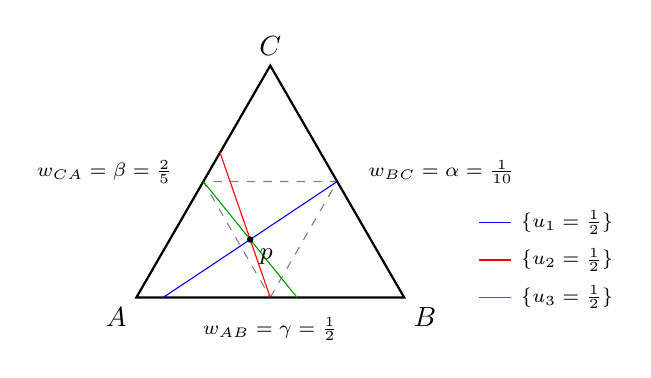
\begin{tikzpicture}[scale=3.4]
  \coordinate (A) at (0,0); \coordinate (B) at (1,0); \coordinate (C) at (0.5,0.866);
  \draw[dashed,gray] (0.5,0) -- (0.75,0.433) -- (0.25,0.433) -- cycle;
  \draw[thick] (A) -- (B) -- (C) -- cycle;
  \draw[blue]  (0.1,0)    -- (0.75,0.433);
  \draw[red]   (0.5,0)    -- (0.3125,0.54125);
  \draw[green!60!black] (0.6,0) -- (0.25,0.433);
  \fill (0.425,0.2165) circle (0.012) node[below right,font=\small] {$p$};
  \node[below left]  at (A) {$A$};
  \node[below right] at (B) {$B$};
  \node[above]       at (C) {$C$};
  \node[below,font=\scriptsize] at (0.5,-0.04) {$w_{AB}=\gamma=\tfrac12$};
  \node[right,font=\scriptsize] at (0.83,0.47) {$w_{BC}=\alpha=\tfrac1{10}$};
  \node[left,font=\scriptsize]  at (0.17,0.47) {$w_{CA}=\beta=\tfrac25$};
  \begin{scope}[shift={(1.28,0.08)}]
    \draw[blue] (0,0.2) -- (0.12,0.2)
      node[right,font=\scriptsize,black] {$\{u_1=\tfrac12\}$};
    \draw[red] (0,0.06) -- (0.12,0.06)
      node[right,font=\scriptsize,black] {$\{u_2=\tfrac12\}$};
    \draw[green!60!black] (0,-0.08) -- (0.12,-0.08)
      node[right,font=\scriptsize,black] {$\{u_3=\tfrac12\}$};
  \end{scope}
\end{tikzpicture}
\caption{The weighted-perimeter witness of Theorem~\ref{thm:wper} at
$p=(\tfrac9{20},\tfrac3{10},\tfrac14)$, i.e.\
$\tau=(\tfrac59,\tfrac45,\tfrac16)$: the three mid-level lines $\{u_i=\tfrac12\}$
concur at $p$, which lies in the open medial triangle (dashed), and $\mu_p$ puts
the indicated masses uniformly on the edges.}
\label{fig:wper}
\end{figure}

Combining necessity (Proposition~\ref{prop:concur}) with the explicit construction
(Theorem~\ref{thm:wper}) yields a \emph{characterization}:
\begin{corollary}\label{cor:iff}
Call a direction triple \emph{cyclic} if its vertex values are
$u_1=(\tau_1,0,1)$, $u_2=(0,1,\tau_2)$, $u_3=(1,\tau_3,0)$ with
$\tau_i\in(0,1)$. A cyclic triple admits a uniform-marginal witness measure if and
only if the three mid-level lines $\{u_i=\tfrac12\}$ concur. In that case the
concurrence point $p$ automatically lies in the open medial triangle
($p_j>0$ and $p_j<\tfrac12$ for all $j$), and the weighted-perimeter measure
$\mu_p$ of Theorem~\ref{thm:wper} is a witness.
\end{corollary}
\begin{proof}
The vertex-value matrix has $\det V=-(1+\tau_1\tau_2\tau_3)\ne0$, so
Proposition~\ref{prop:concur} applies and gives necessity. Conversely, if the lines
concur at $p$ (a point of the affine plane of $\Delta$, so $\sum_jp_j=1$), then $p$
is the unique solution of $Vp=\tfrac12\mathbf1$, which in closed form reads
$2(1+\tau_1\tau_2\tau_3)\,p_A=1-\tau_3(1-\tau_2)$ and cyclically; each right-hand
side is positive for $\tau_i\in(0,1)$, so $p_j>0$, and the identities
$\tfrac12-p_C=\tau_1p_A$, $\tfrac12-p_A=\tau_3p_B$, $\tfrac12-p_B=\tau_2p_C$ give
$p_j<\tfrac12$. Theorem~\ref{thm:wper} then supplies $\mu_p$.
\end{proof}
\begin{remark}
The \emph{anti-cyclic} pattern (all $0$- and $1$-roles exchanged) reduces to the
cyclic one by a reflection of $\Delta$ (a transposition of two vertices), which
maps the medial triangle to itself; Theorem~\ref{thm:wper},
Corollary~\ref{cor:iff} and Theorem~\ref{thm:tight} below hold for it verbatim.
All remaining role assignments are classified by Theorem~\ref{thm:char} below.
\end{remark}

The bound of Theorem~\ref{thm:wper} is in fact \emph{attained} at every member
of the family, and the tight covering is unique --- a two-parameter family of
sharp configurations extending the median rigidity of \S\ref{sec:median}.

The coverage argument below rests on an elementary topological fact, which we
isolate.

\begin{pocketlemma}
Let $H$ be an open convex subset of the plane of $\Delta$ such that
$P:=H\cap\operatorname{int}\Delta\ne\varnothing$ and
$\overline P\cap\partial\Delta$ is finite. Then $H\subseteq\overline\Delta$; in
particular $H$ is bounded.
\end{pocketlemma}

\begin{proof}
Suppose $y\in H\setminus\overline\Delta$, and choose a disk $B\subseteq P$. For
$z\in B$ the segment $[z,y]$ lies in $H$ by convexity and joins
$\operatorname{int}\Delta$ to the complement of $\overline\Delta$; let $w(z)$ be
the first point of $\partial\Delta$ on it, starting from $z$. Then
$[z,w(z))\subseteq H\cap\operatorname{int}\Delta$, so
$w(z)\in\overline P\cap\partial\Delta$, a finite set. But for a fixed boundary
point $w$, every $z$ with $w(z)=w$ lies on the line through $y$ and $w$, and
finitely many lines cannot cover the disk $B$ --- a contradiction.
\end{proof}

\begin{theorem}[tightness and rigidity of the cyclic family]\label{thm:tight}
Let $p$ and $u_1,u_2,u_3$ be as in Theorem~\ref{thm:wper}. Write
$\alpha=1-2p_A$, $\beta=1-2p_B$, $\gamma=1-2p_C$ (the edge masses of $\mu_p$;
$\alpha,\beta,\gamma>0$, $\alpha+\beta+\gamma=1$) and
$S=\alpha\beta+\beta\gamma+\gamma\alpha$. Then the planks $P_i=\{u_i\in I_i\}$
with
\[
I_1=\Bigl[\tfrac{\alpha\gamma}S,\,1-\tfrac{\alpha\beta}S\Bigr],\qquad
I_2=\Bigl[\tfrac{\beta\gamma}S,\,1-\tfrac{\alpha\gamma}S\Bigr],\qquad
I_3=\Bigl[\tfrac{\alpha\beta}S,\,1-\tfrac{\beta\gamma}S\Bigr]
\]
cover $\Delta$, with $\sum\rw
=\tfrac{\beta\gamma}S+\tfrac{\alpha\beta}S+\tfrac{\alpha\gamma}S=1$. Moreover
this is the unique covering of $\Delta$ with $\sum\rw=1$ by three planks of
positive width, one in each of the directions $u_1,u_2,u_3$. At $p$ the centroid
($\alpha=\beta=\gamma=\tfrac13$) it is $[\tfrac13,\tfrac23]^3$, recovering
Theorem~\ref{thm:median}.
\end{theorem}

\begin{proof}
Write $l=(l_1,l_2,l_3)=(\alpha\gamma,\beta\gamma,\alpha\beta)/S$ and
$h=(h_1,h_2,h_3)=\mathbf1-(\alpha\beta,\alpha\gamma,\beta\gamma)/S$, and note
$\tau_1=\frac{\gamma}{1-\alpha}$, $\tau_2=\frac{\beta}{1-\gamma}$,
$\tau_3=\frac{\alpha}{1-\beta}$ from the formulas of Theorem~\ref{thm:wper}. A
direct substitution shows $(l,h)=(\lambda,\rho)$, the first solution of
Proposition~\ref{prop:tilings}; in particular $l_i<\tau_i<h_i$, and the traces
of $P_1,P_2,P_3$ tile all three edges, so $\partial\Delta\subset\bigcup P_i$.

\emph{Step 1: an affine identity.} Let $a_1=\alpha(1-\alpha)$,
$a_2=\gamma(1-\gamma)$, $a_3=\beta(1-\beta)$ and
$\Lambda=a_1u_1+a_2u_2+a_3u_3$. At the vertices:
$\Lambda(A)=a_1\tau_1+a_3=\alpha\gamma+\beta(\alpha+\gamma)=S$,
$\Lambda(B)=a_2+a_3\tau_3=\gamma(\alpha+\beta)+\alpha\beta=S$,
$\Lambda(C)=a_1+a_2\tau_2=\alpha(\beta+\gamma)+\beta\gamma=S$. An affine
function agreeing at three affinely independent points is constant:
$\Lambda\equiv S$ on the plane of $\Delta$. Moreover
$\sum_ia_i=1-(\alpha^2+\beta^2+\gamma^2)=2S$, and expanding (using
$1-\alpha=\beta+\gamma$ etc.)
\[
\textstyle\sum_i a_il_i
=\frac{\alpha^2\gamma(\beta+\gamma)+\beta\gamma^2(\alpha+\beta)
+\alpha\beta^2(\gamma+\alpha)}{S}
=\frac{(\alpha^2\beta^2+\beta^2\gamma^2+\gamma^2\alpha^2)+\alpha\beta\gamma}{S}
=\frac{S^2-\alpha\beta\gamma}{S},
\]
since $S^2=\sum\alpha^2\beta^2+2\alpha\beta\gamma$; the same expansion gives
$\sum_ia_i(1-h_i)=\frac{S^2-\alpha\beta\gamma}S$, whence
$\sum_ia_ih_i=2S-\frac{S^2-\alpha\beta\gamma}S=S+\frac{\alpha\beta\gamma}S$.
Thus
\begin{equation}\label{eq:margin}
\textstyle\sum_i a_il_i=S-\frac{\alpha\beta\gamma}S<S<
S+\frac{\alpha\beta\gamma}S=\sum_i a_ih_i .
\end{equation}

\emph{Step 2: the planks cover $\Delta$.} Suppose not; the uncovered set $U$ is
relatively open (planks are closed) and misses $\partial\Delta$, and it
decomposes as $U=\bigcup_\sigma P_\sigma$ over the eight sign patterns
$\sigma\in\{\mathrm{lo},\mathrm{hi}\}^3$, where $P_\sigma=H_\sigma\cap
\operatorname{int}\Delta$ and $H_\sigma$ is the open convex set
$\{u_i<l_i\ (\sigma_i=\mathrm{lo}),\ u_i>h_i\ (\sigma_i=\mathrm{hi})\}$; write
$c_i$ for the active bound ($l_i$ or $h_i$). We show each $P_\sigma$ is empty.

First, $\overline{P_\sigma}\cap\partial\Delta$ is finite. Indeed, such a point
$x$ satisfies the closed pattern constraints ($u_j(x)\le l_j$ if
$\sigma_j=\mathrm{lo}$, $u_j(x)\ge h_j$ if $\sigma_j=\mathrm{hi}$), and, lying
on the tiled boundary, is covered by some $P_j$, so $u_j(x)\in[l_j,h_j]$;
together these force $u_j(x)=c_j$ for that $j$. Each $u_j$ is affine and
nonconstant on each edge (its two vertex values there are distinct), so
$\{u_j=c_j\}$ meets each edge in at most one point: at most $3\times3=9$ points
in all. By the Pocket Lemma applied to $H_\sigma$ (whose intersection
with $\operatorname{int}\Delta$ is $P_\sigma$),
$H_\sigma\subseteq\overline\Delta$ whenever $P_\sigma\ne\varnothing$; in
particular $H_\sigma$ is bounded.

No two of the lines $\ell_i=\{u_i=c_i\}$ are parallel: $u_i\parallel u_j$ would
force $\tau_1(1-\tau_2)=1$, $\tau_2(1-\tau_3)=1$ or $\tau_3(1-\tau_1)=1$,
impossible for $\tau\in(0,1)^3$. If the three lines are concurrent, $H_\sigma$
is an intersection of three open half-planes whose boundaries pass through one
point, hence empty or an unbounded open cone; boundedness gives
$H_\sigma=\varnothing$. Otherwise $H_\sigma$, if nonempty, is the open triangle
with vertices $v_{ij}=\ell_i\cap\ell_j\in\overline{H_\sigma}
\subseteq\overline\Delta$, and each $v_{ij}$ satisfies the closed constraint in
the third index $k$. Since $\Lambda\equiv S$,
$u_k(v_{ij})=(S-a_ic_i-a_jc_j)/a_k$, so that constraint reads $S\le\sum_ma_mc_m$
if $\sigma_k=\mathrm{lo}$, and $S\ge\sum_ma_mc_m$ if $\sigma_k=\mathrm{hi}$. For
a \emph{mixed} pattern both directions occur, forcing $S=\sum_ma_mc_m$; but then
$u_k(v_{ij})=c_k$, i.e.\ the three lines concur --- excluded. For
$\sigma=(\mathrm{lo},\mathrm{lo},\mathrm{lo})$ we get $S\le\sum a_il_i$, and for
$\sigma=(\mathrm{hi},\mathrm{hi},\mathrm{hi})$, $S\ge\sum a_ih_i$ --- both
contradict \eqref{eq:margin}. Hence $U=\varnothing$: the planks cover, and
$\sum\rw=1$.

\emph{Step 3: uniqueness.} Let $(I_i')$ be any covering with all
$r_i'=|I_i'|>0$ and $\sum r_i'=1$. Since $u_{i\#}\mu_p=\Leb[0,1]$
(Theorem~\ref{thm:wper}), $\mu_p(P_i')=r_i'$, and
$1=\mu_p(\Delta)\le\sum\mu_p(P_i')=1$ forces the planks to partition $\mu_p$
a.e.; as $\mu_p$ has positive uniform density on each edge, the traces tile all
three edges. By Proposition~\ref{prop:tilings}, $(I_i')$ is $(\,[\lambda_i,
\rho_i]\,)=(I_i)$, $(\,[0,\lambda_i]\,)$ or $(\,[\rho_i,1]\,)$. The last two do
not cover $\Delta$: set $\delta=\frac{\alpha\beta\gamma}{2S^2}$ and let
$x^\ast$ be the unique point of the plane with $u_i(x^\ast)=\lambda_i+\delta$
for all $i$ (consistent with $\Lambda\equiv S$ by \eqref{eq:margin} and
$\sum a_i=2S$; unique since $V$ is invertible). Its barycentric coordinates are
\[
x^\ast=\tfrac1{2S^2}\Bigl(\alpha\beta(1-\alpha)(1+\alpha-\beta),\;
\beta\gamma(1-\beta)(\alpha+2\beta),\;
\alpha\gamma(\alpha+\beta)(2-2\alpha-\beta)\Bigr),
\]
all positive: $\alpha,\beta,\gamma>0$ handle the leading factors (with
$1-\alpha=\beta+\gamma>0$), while $1+\alpha-\beta>1-\beta>0$, $\alpha+2\beta>0$,
and $2-2\alpha-\beta=\beta+2\gamma>0$ using $\alpha+\beta+\gamma=1$. So
$x^\ast\in\operatorname{int}\Delta$ and
$u_i(x^\ast)>\lambda_i$ for every $i$: $x^\ast$ is uncovered by
$(\,[0,\lambda_i]\,)$. Symmetrically the point $y^\ast$ with
$u_i(y^\ast)=\rho_i-\delta$, with coordinates
$\frac1{2S^2}\bigl(\alpha\gamma(1-\alpha)(2\alpha+\beta),\,
\alpha\beta(1-\beta)(1+\beta-\alpha),\,
\beta\gamma(\alpha+\beta)(2-\alpha-2\beta)\bigr)$, positive likewise
($2\alpha+\beta>0$, $1+\beta-\alpha>1-\alpha>0$,
$2-\alpha-2\beta=\alpha+2\gamma>0$), is uncovered by
$(\,[\rho_i,1]\,)$. Hence $(I_i')=(I_i)$.
\end{proof}

\begin{remark}
At the centroid, $\delta=\tfrac16$ and both witnesses degenerate to the point
with $u_i\equiv\tfrac12$ --- the centroid itself, recovering the interior
witness used in the proof of Theorem~\ref{thm:median}. The identities of Step~1
and the positivity of the witness coordinates, as well as exact coverage checks
at several family points, are verified symbolically in the archived ancillary
script \texttt{cyclic\_family\_tight\_rigidity.py}.
\end{remark}

Finally, the restriction to cyclic role assignments can be removed altogether.
The plank problem is invariant under the \emph{flip} of a normalized direction,
$u\mapsto1-u$, $I\mapsto1-I$ (the planks, their widths, and uniformity of
marginals are unchanged, and each mid-level line is fixed). Call the edge
joining the $0$- and $1$-vertices of a direction its \emph{full edge}. Flips
reduce every role assignment to one of three shapes, and the existence question
is settled in each:

\begin{theorem}[three-direction characterization]\label{thm:char}
Let $u_1,u_2,u_3$ be normalized directions on $\Delta$, pairwise non-parallel.
A probability measure $\mu$ on $\Delta$ with $u_{i\#}\mu=\Leb[0,1]$ for
$i=1,2,3$ exists if and only if the three mid-level lines $\{u_i=\tfrac12\}$
have a common point $p$. In that case $\sum\rw\ge1$ for every covering of
$\Delta$ by planks parallel to these directions, and exactly one of the
following holds:
\begin{itemize}
\item[(a)] the full edges are pairwise distinct: up to flips the triple is
cyclic, $p$ lies in the open medial triangle, and Theorems~\ref{thm:wper}
and~\ref{thm:tight} apply verbatim (explicit witness $\mu_p$; unique tight
covering);
\item[(b)] all three directions have the same full edge $e$: then $p$ is the
midpoint of $e$, the uniform measure on $e$ is a witness, and the bound follows
from covering $e$ alone (the trivial one-dimensional case recorded in
Theorem~\ref{thm:oned}).
\end{itemize}
\end{theorem}

\begin{proof}
\emph{Necessity.} If $\mu$ exists, its barycenter $p\in\Delta$ satisfies
$u_i(p)=\mathbb E_\mu[u_i]=\tfrac12$ for every $i$ (no invertibility of $V$ is
needed), so the mid-lines concur at $p$.

\emph{Classification.} (1) If the three full edges are distinct, flipping each
direction so that its $(0,1)$-pair is oriented cyclically makes the triple
cyclic; by Corollary~\ref{cor:iff}, concurrence then places $p$ in the open
medial triangle and yields $\mu_p$, and Theorem~\ref{thm:tight} the unique
tight covering. (2) Suppose exactly two directions, say $u_i$ and $u_j$, share
their full edge $e$, and let $x_v$ be the barycentric coordinate of the vertex
$v$ opposite $e$. After a flip, $u_i$ and $u_j$ agree on $e$, so
$u_i-u_j=(\tau_i-\tau_j)x_v$ with $\tau_i\ne\tau_j$ (equality would make them
parallel). Hence $\{u_i=\tfrac12\}\cap\{u_j=\tfrac12\}\subset\{x_v=0\}$, the
line through $e$, on which both mid-lines pass only through the midpoint of
$e$; but the third direction is not full on $e$, its values at the endpoints of
$e$ being $\{0,\tau_k\}$ or $\{\tau_k,1\}$, so its value at the midpoint is
$\tfrac{\tau_k}2$ or $\tfrac{1+\tau_k}2$, never $\tfrac12$. Thus the mid-lines
of such a triple \emph{never} concur; consistently, no witness measure exists
($\mathbb E_\mu[u_i]=\mathbb E_\mu[u_j]=\tfrac12$ would force
$\mathbb E_\mu[x_v]=0$, hence $\operatorname{supp}\mu\subset e$, on which $u_k$
is not onto $[0,1]$). This shape contributes to neither side of the
equivalence. (3) If all three directions share the full edge $e$, then after
flips each restricts to $e$ as the identity parameter, so all mid-lines pass
through the midpoint of $e$ (concurrence always holds), and the uniform
probability measure on $e$ has all three pushforwards equal to $\Leb[0,1]$.
For the bound, a covering of $\Delta$ covers $e$, on which the $i$-th plank
traces an interval of length $r_i$; hence $\sum r_i\ge1$.
\end{proof}

\begin{remark}\label{rem:charscope}
Theorem~\ref{thm:char} answers the existence question of~\cite{Gardner88}
completely for three directions on the triangle. In particular, \emph{within the
uniform-marginal witness-measure approach}, the remaining three-direction case
is that of non-concurrent triples, for which no witness measure can exist. This
is a statement about the reach of the method, not a reduction of
Conjecture~\ref{conj:bang} on the triangle (which concerns arbitrarily many
planks in arbitrary directions).
\end{remark}

\smallskip
The concurrence condition is dimension-agnostic: the cyclic medians of $\Delta^d$
($m_i(e_i)=\tfrac12$, $m_i(e_{i+1})=0$, $m_i(e_{i-1})=1$, else $\tfrac12$) have
row-sums $\tfrac{d+1}2$, hence concur at the centroid in every dimension. (A
caution specific to $d=3$: there $m_{i+2}=1-m_i$, so this literal family collapses
to two directions up to flips; this happens exactly when $d+1$ divides $4$.)
Section~\ref{sec:simplex3} constructs witness measures for a non-degenerate
one-parameter family of concurrent quadruples on $\Delta^3$, extending the
transport method beyond the plane; for $d\ge4$ the question is open
(Problem~\ref{prob:suff}).

\section{The transport defect}\label{sec:defect}
Theorem~\ref{thm:char} says the transport method certifies the full bound
$\sum\rw\ge1$ exactly when the mid-lines concur. We now quantify how the method
degrades off the concurrent locus. Throughout, $u=(u_1,u_2,u_3)$ is a triple of
normalized affine directions on $\Delta$, pairwise non-parallel.

\begin{definition}\label{def:defect}
The \emph{transport defect} of $u$ is
\[
D(u)\;=\;\inf\bigl\{D\ge1:\ \exists\,\mu\in\mathcal P(\Delta)\ \text{with}\
u_{i\#}\mu\le D\cdot\Leb\ \text{on }[0,1]\ \text{for }i=1,2,3\bigr\}.
\]
\end{definition}

\begin{proposition}\label{prop:defect}
(i) The infimum is attained. (ii) Every covering of $\Delta$ by finitely many
planks, each parallel to one of the three directions, satisfies
$\sum\rw\ge 1/D(u)$. (iii) $D(u)=1$ if and only if the mid-lines concur;
otherwise $D(u)>1$. (iv) $D(u)\le2$.
\end{proposition}

\begin{proof}
(i) Take $D_n\downarrow D(u)$ and admissible $\mu_n$; by weak-$*$ compactness of
$\mathcal P(\Delta)$ pass to a limit $\mu$. For every open interval $J$ the set
$u_i^{-1}(J)$ is relatively open in $\Delta$, so
$\mu(u_i^{-1}(J))\le\liminf_n\mu_n(u_i^{-1}(J))\le D(u)|J|$; open intervals
determine the bound $u_{i\#}\mu\le D(u)\Leb$ by outer regularity. (Taking
$J=(-\delta,1+\delta)$ also shows $D(u)\ge1$.)
(ii) For a plank $P$ parallel to $u_i$ with normalized interval $I$,
$\mu(P\cap\Delta)=u_{i\#}\mu(I)\le D(u)\,|I|\le D(u)\rw(P)$; summing over a
covering gives $1\le D(u)\sum\rw$.
(iii) If $D(u)=1$, the attained $\mu$ has $u_{i\#}\mu\le\Leb$ with both sides of
total mass $1$ on $[0,1]$, hence $u_{i\#}\mu=\Leb$, and Theorem~\ref{thm:char}
forces concurrence; the converse is Theorem~\ref{thm:char} again.
(iv) The normalized uniform measure on $\Delta$ satisfies
$\mu(u^{-1}(J))\le2|J|$ for every direction and interval, by the per-plank
estimate in the proof of Theorem~\ref{thm:oned} with $d=2$.
\end{proof}

The necessary condition of Proposition~\ref{prop:concur} can now be made
quantitative. Define the \emph{concurrence defect}
\begin{equation}\label{eq:cdefect}
\delta(u)\;=\;\min_{p\in\Delta}\ \max_{i}\ \bigl|u_i(p)-\tfrac12\bigr|,
\end{equation}
a minimum of a continuous function on a compact set, hence attained; clearly
$\delta(u)=0$ if and only if the mid-lines concur. Moreover $\delta(u)<\tfrac12$:
at any interior $p$ each $u_i(p)\in(0,1)$, since an affine function on $\Delta$
attaining its minimum $0$ at an interior point would be identically $0$.

\begin{proposition}\label{prop:moment}
$D(u)\ \ge\ \dfrac1{1-2\delta(u)}$. In particular, for the facet triple
$u=(\lambda_1,\lambda_2,\lambda_3)$ one has $\delta=\tfrac16$ and $D\ge\tfrac32$.
\end{proposition}

\begin{proof}
Let $\nu$ be a probability measure on $[0,1]$ with $\nu\le D\Leb$ and
distribution function $F(t)\le\min(1,Dt)$. Its mean is
$\int_0^1(1-F)\ge\int_0^1\max(0,1-Dt)\,dt=\tfrac1{2D}$, and by the mirror
argument the mean lies in $[\tfrac1{2D},\,1-\tfrac1{2D}]$. If $\mu$ is
admissible for $D$ and $p$ is its barycenter, then $p\in\Delta$ and the mean of
$u_{i\#}\mu$ is $u_i(p)$, so
$\delta(u)\le\max_i|u_i(p)-\tfrac12|\le\tfrac12-\tfrac1{2D}$, which rearranges
to the claim. For the facets, $\sum_i\lambda_i(p)=1$ forces some
$\lambda_i(p)\le\tfrac13$, so $\delta\ge\tfrac16$; the centroid attains
$\tfrac16$.
\end{proof}

At the facets the moment bound is exact:

\begin{theorem}\label{thm:facetdefect}
For the facet triple, $D(\lambda_1,\lambda_2,\lambda_3)=\tfrac32$. The infimum
is attained by the uniform probability measure on the perimeter of the inscribed
triangle with vertices
\[
P_0=(0,\tfrac13,\tfrac23),\qquad P_1=(\tfrac23,0,\tfrac13),\qquad
P_2=(\tfrac13,\tfrac23,0),
\]
whose three marginals all equal $\tfrac32\cdot\mathbf 1_{[0,2/3]}$.
\end{theorem}

\begin{proof}
The lower bound is Proposition~\ref{prop:moment}. For the upper bound give each
side of the loop mass $\tfrac13$, uniformly in the parameter. The coordinate
$\lambda_1$ is affine on each side, with values $0\to\tfrac23$ on $P_0P_1$
(density $\tfrac12$ on $[0,\tfrac23]$), $\tfrac23\to\tfrac13$ on $P_1P_2$
(density $1$ on $[\tfrac13,\tfrac23]$), and $\tfrac13\to0$ on $P_2P_0$ (density
$1$ on $[0,\tfrac13]$); the total is $\tfrac32$ on $[0,\tfrac23]$. The loop is
invariant under the cyclic rotation of $\Delta$, so the same holds for
$\lambda_2,\lambda_3$.
\end{proof}

\begin{figure}[ht]
\centering
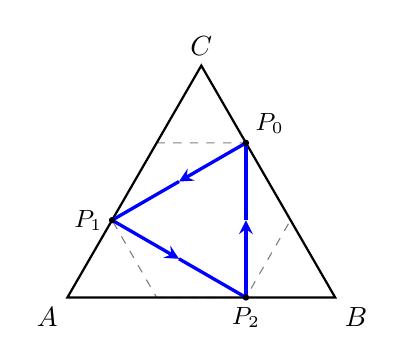
\begin{tikzpicture}[scale=3.4]
  \coordinate (A) at (0,0); \coordinate (B) at (1,0); \coordinate (C) at (0.5,0.866);
  \draw[dashed,gray] (0.3333,0) -- (0.6667,0) -- (0.8333,0.2887)
       -- (0.6667,0.5773) -- (0.3333,0.5773) -- (0.1667,0.2887) -- cycle;
  \draw[thick] (A) -- (B) -- (C) -- cycle;
  \draw[very thick,blue,-stealth] (0.6667,0.5773) -- (0.4167,0.4330);
  \draw[very thick,blue] (0.4167,0.4330) -- (0.1667,0.2887);
  \draw[very thick,blue,-stealth] (0.1667,0.2887) -- (0.4167,0.14435);
  \draw[very thick,blue] (0.4167,0.14435) -- (0.6667,0);
  \draw[very thick,blue,-stealth] (0.6667,0) -- (0.6667,0.28865);
  \draw[very thick,blue] (0.6667,0.28865) -- (0.6667,0.5773);
  \fill (0.6667,0.5773) circle (0.012) node[above right,font=\small] {$P_0$};
  \fill (0.1667,0.2887) circle (0.012) node[left,font=\small] {$P_1$};
  \fill (0.6667,0) circle (0.012) node[below,font=\small] {$P_2$};
  \node[below left]  at (A) {$A$};
  \node[below right] at (B) {$B$};
  \node[above]       at (C) {$C$};
\end{tikzpicture}
\caption{The witness of Theorem~\ref{thm:facetdefect}: the uniform measure on
the inscribed loop $P_0P_1P_2$ (mass $\tfrac13$ per side) has all three
marginals equal to $\tfrac32\cdot\mathbf1_{[0,2/3]}$, so $D=\tfrac32$ for the
facet triple. Dashed: the hexagon $\{\max_i\lambda_i\le\tfrac23\}$, whose
alternate vertices the loop connects.}
\label{fig:loop}
\end{figure}

\begin{remark}\label{rem:complement}
Theorem~\ref{thm:facetdefect} makes precise the complementarity of the two
methods in this paper: for facet directions the tiling argument of
Theorem~\ref{thm:facet} certifies the sharp bound $1$, while the transport
method cannot certify more than $1/D=\tfrac23$ --- and now provably certifies
exactly that. Conversely, for the concurrent cyclic triples the transport bound is
sharp (Theorems~\ref{thm:wper} and~\ref{thm:tight}) where no facet tiling is
available.
\end{remark}

Near the concurrent locus the defect is small, with an explicit modulus; this
gives bounds beyond the general constant of~\cite{BY26} on open sets of
non-concurrent triples, for coverings in the corresponding direction families
(see Remark~\ref{rem:beyond}).

\begin{theorem}\label{thm:defectstab}
Let $\tau^*\in(0,1)^3$ be a concurrent cyclic parameter with edge masses
$(\alpha,\beta,\gamma)$ as in Theorem~\ref{thm:wper}, and let
$m=\min_i\min(\tau_i^*,1-\tau_i^*)$. If $\tau\in(0,1)^3$ is a cyclic parameter
with $\varepsilon:=\max_i|\tau_i-\tau_i^*|<m$, then
\[
D(u_\tau)\ \le\ 1+\frac{\varepsilon}{m(m-\varepsilon)},
\qquad\text{hence}\qquad
\sum\rw\ \ge\ 1-\frac{\varepsilon}{m(m-\varepsilon)}
\]
for every covering of $\Delta$ by planks parallel to the directions of $\tau$.
\end{theorem}

\begin{proof}
Keep the \emph{frozen} weights: let $\mu$ be the measure with masses
$(\gamma,\alpha,\beta)$ on the edges $(AB,BC,CA)$, uniform in the parameter, and
push it forward by the \emph{perturbed} directions. For $u_1$ (vertex values
$(\tau_1,0,1)$) the marginal density is $\alpha+\gamma/\tau_1$ on $[0,\tau_1]$
and $\alpha+\beta/(1-\tau_1)$ on $[\tau_1,1]$; at $\tau_1^*$ both equal $1$ by
the choice of weights in Theorem~\ref{thm:wper}. Subtracting,
\[
\Bigl(\alpha+\frac{\gamma}{\tau_1}\Bigr)-1
=\frac{\gamma\,(\tau_1^*-\tau_1)}{\tau_1\tau_1^*},\qquad
\Bigl(\alpha+\frac{\beta}{1-\tau_1}\Bigr)-1
=\frac{\beta\,(\tau_1-\tau_1^*)}{(1-\tau_1)(1-\tau_1^*)},
\]
and since $\gamma,\beta\le1$, $\tau_1^*\ge m$, $1-\tau_1^*\ge m$ and
$\tau_1,1-\tau_1\ge m-\varepsilon$, both deviations are at most
$\varepsilon/(m(m-\varepsilon))$ in absolute value; the same computation applies
to $u_2,u_3$. Hence $u_{i\#}\mu\le(1+\varepsilon/(m(m-\varepsilon)))\Leb$ for
all $i$, and Proposition~\ref{prop:defect}(ii) with
$1/(1+x)\ge1-x$ gives the covering bound.
\end{proof}

\begin{corollary}\label{cor:beyond}
Every covering of $\Delta$ by planks parallel to the directions of a cyclic
parameter $\tau$ with $\max_i|\tau_i-\tfrac12|\le\tfrac1{60}$ satisfies
\[
\sum\rw\ \ge\ \tfrac{27}{29}\ >\ 4\sqrt3-6 .
\]
\end{corollary}

\begin{proof}
Apply Theorem~\ref{thm:defectstab} with $\tau^*=(\tfrac12,\tfrac12,\tfrac12)$
(the medians, concurrent with $\alpha=\beta=\gamma=\tfrac13$), $m=\tfrac12$,
$\varepsilon=\tfrac1{60}$: the loss is
$\frac{1/60}{(1/2)(1/2-1/60)}=\tfrac2{29}$. The comparison
$\tfrac{27}{29}>4\sqrt3-6$ is $(\tfrac{201}{29})^2=\tfrac{40401}{841}>48$, i.e.\
$40401>40368$.
\end{proof}

\begin{remark}\label{rem:beyond}
The set of triples covered by Corollary~\ref{cor:beyond} is a full-dimensional
neighbourhood in the three-parameter space of cyclic triples, and the concurrent
ones form a codimension-one subset of it: the corollary is a bound strictly
inside non-concurrent territory, where by Theorem~\ref{thm:char} no witness
measure exists and $\sum\rw\ge1$ remains open. We stress the honest comparison:
the bound $4\sqrt3-6$ of~\cite{BY26} is uniform over \emph{all} direction
triples, while ours improves on it only on this neighbourhood; far from the
concurrent locus the moment bound (Proposition~\ref{prop:moment}) shows the
transport method degrades irreparably --- at the facets down to $\tfrac23$.
\end{remark}

\begin{remark}\label{rem:sandwich}
$D(u)$ is computable to certified precision by exact linear programming over
skeleton measures. For example, for the (non-concurrent) cyclic parameter
$\tau=(\tfrac{13}{25},\tfrac12,\tfrac12)$ one gets
$\tfrac{225}{224}\le D(u_\tau)\le\tfrac{112}{111}$: the lower bound from
Proposition~\ref{prop:moment} with $\delta=\tfrac1{450}$, the upper from the
optimal edge-skeleton measure. Whether the moment bound is exact off the
symmetric cases --- as it is at the facets and, trivially, on the concurrent
locus --- we leave open; the ancillary script
\texttt{transport\_defect.py} contains the exact computations.
\end{remark}

\section{A witness family on the 3-simplex}\label{sec:simplex3}
Let $\Delta^3=\operatorname{conv}(e_1,\dots,e_4)$ and fix $\sigma\in(0,1)$.
Define four normalized affine directions by their vertex values (indices mod
$4$):
\begin{equation}\label{eq:sigma-family}
u_i(e_i)=0,\qquad u_i(e_{i+1})=1,\qquad u_i(e_{i+2})=\sigma,\qquad
u_i(e_{i+3})=1-\sigma .
\end{equation}
Each row sums to $2$, so the mid-hyperplanes $\{u_i=\tfrac12\}$ concur at the
centroid (Proposition~\ref{prop:concur}); at $\sigma=\tfrac12$ the
$\{u_i=\tfrac12\}$ are the ``median'' planes through an edge and the midpoint of
the opposite edge. The four directions are pairwise non-parallel for every
$\sigma$: an affine relation $u_{i+1}=c\,u_i+e$ forces, comparing vertex values,
$(1-\sigma)^2=1$, and $u_{i+2}=c\,u_i+e$ forces $2\sigma(1-\sigma)=0$, both
impossible on $(0,1)$.

\begin{theorem}\label{thm:simplex3}
Let $\sigma\in(0,\tfrac12]$ and set
\[
a(\sigma)=\frac{(1-\sigma)(1-2\sigma)}{2(\sigma^2-4\sigma+2)},\qquad
b(\sigma)=\frac{\sigma(2-3\sigma)}{2(\sigma^2-4\sigma+2)} .
\]
The measure $\mu_\sigma$ placing mass $a(\sigma)$ on each of the four cycle
edges $e_ie_{i+1}$ and mass $b(\sigma)$ on each of the two diagonals
$e_1e_3$, $e_2e_4$, uniformly in the parameter on each edge, is a probability
measure on the $1$-skeleton of $\Delta^3$ with
\[
u_{i\#}\mu_\sigma=\Leb[0,1]\qquad\text{for }i=1,\dots,4 .
\]
Consequently every covering of $\Delta^3$ by planks parallel to these four
directions satisfies $\sum\rw\ge1$. For $\sigma\in(\tfrac12,1)$ the same holds
with the flip $u\mapsto1-u$ (which exchanges $\sigma\leftrightarrow1-\sigma$ and
reverses the cyclic order). Moreover $\mu_\sigma$ is the unique cyclically
invariant edge-uniform witness, and at $\sigma=\tfrac12$ (where $a=0$,
$b=\tfrac12$) it is the unique witness supported on the $1$-skeleton at all.
\end{theorem}

\begin{proof}
Positivity of the weights on $(0,\tfrac12]$: the roots of $\sigma^2-4\sigma+2$
are $2\pm\sqrt2$, so the denominator is positive on
$(0,\tfrac12]\subset(0,2-\sqrt2)$, and the numerators are nonnegative there
(vanishing only at $\sigma=\tfrac12$, where the middle piece below is empty).

By the cyclic symmetry of \eqref{eq:sigma-family} it suffices to compute the
$u_1$-marginal. The six edges push forward as follows ($\sigma<\tfrac12$; each
edge uniform, mass as assigned): $e_1e_2$, values $0\to1$, density $a$ on
$[0,1]$; $e_2e_3$, values $1\to\sigma$, density $a/(1-\sigma)$ on $[\sigma,1]$;
$e_3e_4$, values $\sigma\to1-\sigma$, density $a/(1-2\sigma)$ on
$[\sigma,1-\sigma]$; $e_4e_1$, values $1-\sigma\to0$, density $a/(1-\sigma)$ on
$[0,1-\sigma]$; $e_1e_3$, values $0\to\sigma$, density $b/\sigma$ on
$[0,\sigma]$; $e_2e_4$, values $1\to1-\sigma$, density $b/\sigma$ on
$[1-\sigma,1]$. The total density is
\[
a+\frac{a}{1-\sigma}+\frac b\sigma\ \text{ on }[0,\sigma]\ \text{and on }
[1-\sigma,1],\qquad
a+\frac{2a}{1-\sigma}+\frac{a}{1-2\sigma}\ \text{ on }[\sigma,1-\sigma],
\]
and a direct expansion shows both expressions equal $1$ exactly for the stated
$a(\sigma),b(\sigma)$; the total mass $4a+2b=1$ is then automatic, since
pushforward preserves mass. The covering bound follows as in
Proposition~\ref{prop:defect}(ii) with $D=1$. Uniqueness among cyclically
invariant edge-uniform measures: the middle-piece equation determines $a$ and
either outer equation then determines $b$. (Exact linear algebra, recorded in
the ancillary files, shows uniqueness among \emph{all} edge-uniform weightings.)
At $\sigma=\tfrac12$ the values \eqref{eq:sigma-family}
make $u_i$ \emph{constant} ($\equiv\tfrac12$) on the cycle edge
$e_{i+2}e_{i+3}$; any skeleton measure giving positive mass to a cycle edge
would push forward to an atom at $\tfrac12$ under the corresponding direction,
so all four cycle-edge masses vanish, and on the two diagonals each direction is
affine onto $[0,\tfrac12]$ or $[\tfrac12,1]$, forcing the uniform density
$\tfrac12+\tfrac12$ split.
\end{proof}

\begin{proposition}\label{prop:skelobstruction}
For $d\ge4$, consider the cyclic medians of $\Delta^d$: $u_i(e_i)=0$,
$u_i(e_{i+1})=1$ and $u_i(e_j)=\tfrac12$ otherwise (indices mod $d+1$). Then
\emph{every} edge $e_je_k$ of $\Delta^d$ is constant for some direction, and
consequently no measure supported on the $1$-skeleton has uniform marginals for
all $d+1$ directions.
\end{proposition}

\begin{proof}
Fix an edge $\{j,k\}$. Removing $j,k$ from the cycle on $d+1\ge5$ vertices
leaves at least three vertices in at most two arcs, so some arc contains two
cyclically consecutive vertices $\{m,m+1\}$ disjoint from $\{j,k\}$; then $u_m$
takes the value $\tfrac12$ at both $e_j$ and $e_k$, hence is constant on the
edge. A skeleton measure with positive mass on $e_je_k$ pushes forward under
$u_m$ to a measure with an atom at $\tfrac12$, which is not $\le D\cdot\Leb$ for
any finite $D$; so all edge masses vanish.
\end{proof}

\begin{remark}
The obstruction is specific to the all-$\tfrac12$ interior values; whether
distinct interior values (the $d\ge4$ analogue of
\eqref{eq:sigma-family}) revive the skeleton, or the mass must move to
$2$-faces, is open and part of Problem~\ref{prob:suff}.
\end{remark}

\section{A normalizer obstruction}\label{sec:nogo}
For a direction $u$ let $\ell_K(u)$ be the length of the longest chord of $K$
parallel to $u$; always $\ell_K(u)\le\wid_K(u)$. Bakaev--Yehudayoff's chord bound
$\sum_i\wid(P_i)/\ell_K(u_i)\ge1$~\cite{BY26} follows from Bang's sign argument
via the chord lemma. Consider interpolating the normalizer,
$N_c=(1-c)\ell+c\,\wid$, $c\in[0,1]$: $N_c=\ell$ at $c=0$ (chord bound) and
$N_c=\wid$ at $c=1$ (Conjecture~\ref{conj:bang}).
\begin{proposition}\label{thm:nogo}
For a convex body $K$, a direction $u$ with $\|u\|=a/2$ and
$\ell=\ell_K(u)\ge a$, the body $(K-u)\cap(K+u)$ contains a homothet of $K$ of
ratio $(\ell-a)/\ell$ \cite[Lem.~2.3]{Verreault}, and this ratio is sharp: for
$K$ a segment of length $\ell$ parallel to $u$, the set $(K-u)\cap(K+u)$ is a
segment of length exactly $\ell-a$, and no homothet of $K$ of larger ratio fits
in it.
\end{proposition}
\begin{proof}
The containment is \cite[Lem.~2.3]{Verreault}. For sharpness let
$K=[y,z]$ with $z-y=\ell\,\hat u$ and $u=\tfrac a2\hat u$: then
$K-u=[y-\tfrac a2\hat u,\,z-\tfrac a2\hat u]$ and
$K+u=[y+\tfrac a2\hat u,\,z+\tfrac a2\hat u]$, whose intersection is
$[y+\tfrac a2\hat u,\,z-\tfrac a2\hat u]$, a segment of length $\ell-a$; a
homothet of $K$ contained in it has ratio at most $(\ell-a)/\ell$.
\end{proof}
\begin{remark}[methodological obstruction]\label{rem:nogo}
The reading of Proposition~\ref{thm:nogo} that matters here is about the
\emph{sign argument}: iterating the chord lemma over the directions $u_j$
places a Bang-system witness $x_0+\sum_j\pm u_j$ as soon as
$\sum_j\wid(P_j)/\ell_j<1$, which is how the chord bound
$\sum\wid(P_j)/\ell_j\ge1$ of~\cite{BY26} follows. The movement budget in
direction $u$ is governed by the homothety ratio of
Proposition~\ref{thm:nogo}, which is exactly $(\ell-a)/\ell$ and cannot be
stretched: the placement route proves the bound for the normalizer
$N=\ell$ and for no direction-normalizer $N>\ell$; in particular it does not
establish $\sum_i\wid(P_i)/N_c(u_i)\ge1$ for any $c>0$. This does \emph{not}
show the latter inequality false; it shows this route cannot prove it. Beating
$2/(1+\sqrt d)$ by such a normalizer therefore requires a witness that is not a
Bang-system point, i.e.\ one exploiting the coupling of the covering ---
consistent with the sharpness of~\cite{BY26} for the cube.
\end{remark}

\section{Open problems}
\begin{problem}
The three-plank case for non-concurrent tilted triples on the triangle:
Theorem~\ref{thm:char} settles the concurrent case, and shows that for
non-concurrent triples no witness measure exists, so a different mechanism is
needed there. (This is the three-plank sub-problem; Conjecture~\ref{conj:bang}
for the triangle concerns coverings by arbitrarily many planks and is not
reduced to it.)
\end{problem}
\begin{problem}\label{prob:suff}
Theorem~\ref{thm:char} settles the existence of uniform-marginal witness
measures for three directions on the triangle, and Theorem~\ref{thm:simplex3}
gives an affirmative one-parameter family of concurrent quadruples on
$\Delta^3$. For $d\ge3$ the concurrence condition of
Proposition~\ref{prop:concur} remains necessary; is it sufficient for $d+1$
directions on $\Delta^d$? For the cyclic medians of $\Delta^d$ with $d\ge4$,
any witness must vanish on the $1$-skeleton
(Proposition~\ref{prop:skelobstruction}); the first open cases are supports on
$2$-faces, or interior vertex values as in \eqref{eq:sigma-family}.
\end{problem}
\begin{problem}\label{prob:defect}
Is the moment bound of Proposition~\ref{prop:moment} always exact, i.e.\ does
$D(u)=1/(1-2\delta(u))$ hold for every pairwise non-parallel triple on the
triangle (as it does at the facets and on the concurrent locus)? In particular,
is $\sup_uD(u)=\tfrac32$, attained at the facet triple? A small exact sweep
(ancillary files) finds no triple with $\delta(u)>\tfrac16$.
\end{problem}
\begin{problem}
Whether $\sum\wid(P_i)/N_c(u_i)\ge1$ holds for some $c>0$ (a coupling certificate),
which would improve the general bound past $2/(1+\sqrt d)$.
\end{problem}

\appendix
\section{Edge tilings of cyclic triples}\label{app:tilings}

Throughout, $u_1=(\tau_1,0,1)$, $u_2=(0,1,\tau_2)$, $u_3=(1,\tau_3,0)$ is a
cyclic triple with arbitrary $\tau_1,\tau_2,\tau_3\in(0,1)$ (\emph{no}
concurrence is assumed), and $I_i=[l_i,h_i]\subset[0,1]$, $l_i<h_i$, are three
intervals. Say $(I_1,I_2,I_3)$ satisfies the \emph{edge-tiling conditions} if on
each edge of $\Delta$ the traces $T_i=\{x\in\text{edge}: u_i(x)\in I_i\}$ cover
the edge and have pairwise disjoint interiors. Indices are mod~$3$.

\begin{proposition}\label{prop:tilings}
For every $\tau\in(0,1)^3$ the edge-tiling conditions have exactly three
solutions: with
\[
\lambda_i=\frac{\tau_i\bigl(1-\tau_{i+1}(1-\tau_{i+2})\bigr)}{1+\tau_1\tau_2\tau_3},
\qquad
\rho_i=\frac{1-\tau_{i+2}(1-\tau_i)}{1+(1-\tau_1)(1-\tau_2)(1-\tau_3)},
\]
they are $\bigl([\lambda_i,\rho_i]\bigr)_i$, $\bigl([0,\lambda_i]\bigr)_i$, and
$\bigl([\rho_i,1]\bigr)_i$. One has $0<\lambda_i<\tau_i<\rho_i<1$ for all $i$ and
all $\tau$. For $\tau_i\equiv\tfrac12$ (the medians) the solutions are
$[\tfrac13,\tfrac23]^3$, $[0,\tfrac13]^3$, $[\tfrac23,1]^3$.
\end{proposition}

\subsection*{Setup}
Parametrize the edges by $t\in[0,1]$ in the orientations $A\!\to\!B$,
$B\!\to\!C$, $C\!\to\!A$. From the vertex values, each edge sees one direction
with values $[0,\tau_c]$ (the \emph{low} direction $c$, $u_c(t)=\tau_c(1-t)$),
one with values $[0,1]$ (the \emph{full} direction $f$, $u_f(t)=t$), and one
with values $[\tau_g,1]$ (the \emph{high} direction $g$,
$u_g(t)=1-(1-\tau_g)t$), with roles
\[
(c,f,g)=(1,2,3)\ \text{on } AB,\qquad (3,1,2)\ \text{on } BC,\qquad
(2,3,1)\ \text{on } CA .
\]
Inverting, the traces on an edge with roles $(c,f,g)$ are
\begin{equation}\label{eq:traces}
\begin{aligned}
T_c&=\Bigl[\max\bigl(0,1-\tfrac{h_c}{\tau_c}\bigr),\,1-\tfrac{l_c}{\tau_c}\Bigr]
\ \ (\text{nondegenerate iff }l_c<\tau_c),\qquad T_f=[l_f,h_f],\\
T_g&=\Bigl[\tfrac{1-h_g}{1-\tau_g},\,
\min\bigl(1,\tfrac{1-l_g}{1-\tau_g}\bigr)\Bigr]
\ \ (\text{nondegenerate iff }h_g>\tau_g).
\end{aligned}
\end{equation}
Classify each $I_i$ by its position relative to $\tau_i$: type $\mathrm L$ if
$h_i\le\tau_i$, type $\mathrm R$ if $l_i\ge\tau_i$, type $\mathrm M$ if
$l_i<\tau_i<h_i$; every $I_i$ is of exactly one type. Two elementary
observations, used throughout:

\emph{(O1)} If $I_c$ is of type $\mathrm M$ then $T_c=[0,\,1-l_c/\tau_c]$ (it
contains the left endpoint); if $I_c$ is of type $\mathrm R$ then $T_c$ is
degenerate (a point or empty). Dually, if $I_g$ is of type $\mathrm M$ then
$T_g=[(1-h_g)/(1-\tau_g),\,1]$; if $I_g$ is of type $\mathrm L$ then $T_g$ is
degenerate.

\emph{(O2)} The tiling condition is insensitive to degenerate traces: a
degenerate trace covers at most one point, and since the nondegenerate traces
are finitely many closed sets whose union contains $[0,1]$ minus finitely many
points, that union is all of $[0,1]$. So on each edge the \emph{nondegenerate}
traces tile $[0,1]$; in particular, finitely many closed intervals of positive
length with disjoint interiors covering $[0,1]$ abut consecutively from $0$
to~$1$. Consequently the case analysis below requires no genericity in $\tau$
or in the endpoints: whenever an endpoint coincidence (e.g.\ $h_i=\tau_i$ or
$l_i=\tau_i$) makes a trace degenerate, (O2) discards it, and every case
argument uses only the defining non-strict inequalities of the types.

\subsection*{Symmetries}
Two operations act on the data $(\tau;I_1,I_2,I_3)$ and transport edge-tilings
to edge-tilings.

The \emph{rotation} $\varrho$ is induced by the affine map $A\to B\to C\to A$
of $\Delta$: it carries the cyclic triple with parameter
$(\tau_1,\tau_2,\tau_3)$ to the one with parameter $(\tau_2,\tau_3,\tau_1)$ and
acts by $(I_1,I_2,I_3)\mapsto(I_2,I_3,I_1)$, shifting type vectors cyclically.

The \emph{reflected flip} $\varsigma$ is the affine reflection of $\Delta$
swapping $B$ and $C$, composed with the flip $s\mapsto1-s$ of each normalized
direction. The flip replaces each $u_i$ by $1-u_i$ and each $I_i$ by $1-I_i$
($1-[l,h]=[1-h,1-l]$), leaving every plank, every width, every trace and the
tiling conditions unchanged; the reflection then restores the cyclic
normalization (value $0$ and $1$ at the prescribed vertices), and the composite
carries the parameter $(\tau_1,\tau_2,\tau_3)$ to
$(1-\tau_1,\,1-\tau_3,\,1-\tau_2)$, acting by
$(I_1,I_2,I_3)\mapsto(1-I_1,\,1-I_3,\,1-I_2)$; on type vectors it acts by
$(X_1,X_2,X_3)\mapsto(\bar X_1,\bar X_3,\bar X_2)$, where the bar exchanges
$\mathrm L\leftrightarrow\mathrm R$ and fixes $\mathrm M$.

One checks $\varsigma^2=\mathrm{id}$ and
$\varsigma\varrho\varsigma=\varrho^{-1}$, so
$G=\langle\varrho,\varsigma\rangle$ is a group of order $6$ (isomorphic to
$S_3$). Each $g\in G$ maps the edge-tiling problem with parameter $\tau$
\emph{bijectively} onto the problem with parameter $g(\tau)$. Since
Proposition~\ref{prop:tilings} is proved for \emph{all} $\tau\in(0,1)^3$
simultaneously, it suffices to treat one representative of each $G$-orbit of
the $27$ type vectors $(X_1,X_2,X_3)\in\{\mathrm L,\mathrm M,\mathrm R\}^3$:
\[
\mathrm{MMM};\quad \mathrm{LLL}\ (\sim\mathrm{RRR});\quad \mathrm{MML};\quad
\mathrm{LLM};\quad \mathrm{LLR};\quad \mathrm{LMR};\quad \mathrm{LRM}
\]
(orbit sizes $1,2,6,6,6,3,3$, summing to $27$).

\subsection*{Case MMM}
By (O1), on every edge $T_c=[0,\,1-l_c/\tau_c]$ and
$T_g=[(1-h_g)/(1-\tau_g),\,1]$, both nondegenerate, and $T_f$ has positive
length. Disjointness of interiors forces $T_f$ inside the gap between them, and
covering forces the abutments
\[
l_f=1-\frac{l_c}{\tau_c},\qquad h_f=\frac{1-h_g}{1-\tau_g}.
\]
Reading this on the three edges gives two decoupled cyclic systems,
\[
l_2=1-\frac{l_1}{\tau_1},\quad l_1=1-\frac{l_3}{\tau_3},\quad
l_3=1-\frac{l_2}{\tau_2};
\qquad
h_1=\frac{1-h_2}{1-\tau_2},\quad h_2=\frac{1-h_3}{1-\tau_3},\quad
h_3=\frac{1-h_1}{1-\tau_1}.
\]
Each system composes three decreasing affine maps, so the composite self-map
(of $l_1$, resp.\ $h_1$) is affine with negative slope
($-1/(\tau_1\tau_2\tau_3)$, resp.\ $-1/\prod(1-\tau_i)$), hence has a unique
fixed point: the solutions are $l_i=\lambda_i$, $h_i=\rho_i$ (direct
substitution verifies the formulas; e.g.\
$1-\lambda_1/\tau_1
=\bigl(\tau_1\tau_2\tau_3+\tau_2(1-\tau_3)\bigr)/(1+\tau_1\tau_2\tau_3)
=\lambda_2$). The chain
$0<\lambda_i<\tau_i<\rho_i<1$ reduces to
$\tau_{i+1}(\tau_{i+2}-1)<\tau_1\tau_2\tau_3$ and $\tau_i(1-\tau_{i+1})<1$,
both automatic; so the solution is of type MMM and, by construction, tiles each
edge as $[0,l_f]\cup[l_f,h_f]\cup[h_f,1]$ (Figure~\ref{fig:tiling}).

\begin{figure}[ht]
\centering
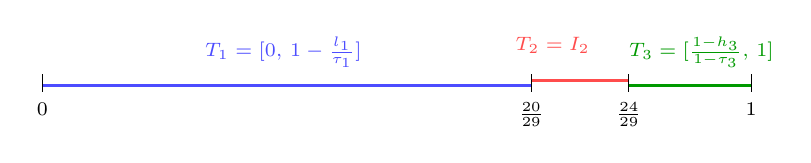
\begin{tikzpicture}[xscale=9,yscale=1]
  \draw[very thick,blue!70]  (0,0)      -- (0.6897,0);
  \draw[very thick,red!70]   (0.6897,0.06) -- (0.8276,0.06);
  \draw[very thick,green!60!black] (0.8276,0) -- (1,0);
  \foreach \x in {0,0.6897,0.8276,1} \draw (\x,-0.08) -- (\x,0.14);
  \node[below,font=\scriptsize] at (0,-0.1) {$0$};
  \node[below,font=\scriptsize] at (0.6897,-0.1) {$\tfrac{20}{29}$};
  \node[below,font=\scriptsize] at (0.8276,-0.1) {$\tfrac{24}{29}$};
  \node[below,font=\scriptsize] at (1,-0.1) {$1$};
  \node[above,font=\scriptsize,blue!70] at (0.34,0.1)
    {$T_1=[0,\,1-\frac{l_1}{\tau_1}]$};
  \node[above,font=\scriptsize,red!70] at (0.72,0.28) {$T_2=I_2$};
  \node[above,font=\scriptsize,green!60!black] at (0.93,0.1)
    {$T_3=[\frac{1-h_3}{1-\tau_3},\,1]$};
\end{tikzpicture}
\caption{The MMM edge tiling on $AB$ (roles $(c,f,g)=(1,2,3)$) for the running
example $\tau=(\tfrac59,\tfrac45,\tfrac16)$: the traces of
$I=([\tfrac5{29},\tfrac{25}{29}],[\tfrac{20}{29},\tfrac{24}{29}],
[\tfrac4{29},\tfrac9{29}])$ abut at $\tfrac{20}{29}$ and $\tfrac{24}{29}$ and
tile $[0,1]$, as forced in Case MMM.}
\label{fig:tiling}
\end{figure}

\subsection*{Case LLL}
All $T_g$ are degenerate, so each edge is tiled by
$T_c=[1-h_c/\tau_c,\,1-l_c/\tau_c]$ (the full image, as $I_c\subset[0,\tau_c]$)
and $T_f=I_f$ with $h_f\le\tau_f<1$. The tile containing $1$ must be $T_c$,
forcing $l_c=0$. If $h_c=\tau_c$ then $T_c=[0,1]$ and $T_f$ has empty interior,
impossible; so $T_f$ contains $0$ ($l_f=0$) and abuts $T_c$:
$h_f=1-h_c/\tau_c$. On the three edges: $l_i=0$ for all $i$, and the $h_i$
satisfy the \emph{same} cyclic system as the $l_i$ in case MMM, so
$h_i=\lambda_i$, giving $\bigl([0,\lambda_i]\bigr)_i$ (type $\mathrm L$ since
$\lambda_i<\tau_i$). Applying the reflection symmetry, the orbit representative
RRR yields the unique solution $h_i=1$, $l_i=\rho_i$, i.e.\
$\bigl([\rho_i,1]\bigr)_i$; equivalently, the $l_i$ satisfy the same cyclic
system as the $h_i$ in case MMM.

\subsection*{Case MML \textup(impossible\textup)}
On $AB$: $T_3$ is degenerate ($I_3$ of type $\mathrm L$), so $[0,1]$ is tiled
by $T_1=[0,\,1-l_1/\tau_1]$ (O1) and $T_2=I_2$. If $1\in T_1$ then $T_1=[0,1]$
and $T_2$ has empty interior, impossible; so $h_2=1$. Then on $BC$ the high
trace \eqref{eq:traces} is
$T_2=[\tfrac{1-h_2}{1-\tau_2},\min(1,\tfrac{1-l_2}{1-\tau_2})]=[0,1]$ (as
$h_2=1$ and $l_2<\tau_2$), leaving the full trace $T_1=I_1$ (positive length)
with empty interior --- contradiction.

\subsection*{Case LLM \textup(impossible\textup)}
On $BC$ ($(c,f,g)=(3,1,2)$): the high trace is degenerate ($I_2$ of type
$\mathrm L$), so $[0,1]$ is tiled by $T_3=[0,\,1-l_3/\tau_3]$ (O1, $I_3$ of
type $\mathrm M$) and $T_1=I_1$ with $h_1\le\tau_1<1$. The tile containing $1$
must be $T_3$, so $l_3=0$ and $T_3=[0,1]$, leaving $T_1$ with empty interior
--- contradiction.

\subsection*{Case LLR \textup(impossible\textup)}
On $BC$ both compressed traces are degenerate ($I_3$ of type $\mathrm R$ gives
a degenerate low trace, $I_2$ of type $\mathrm L$ a degenerate high trace), so
$T_1=I_1$ alone tiles $[0,1]$, forcing $h_1=1>\tau_1$ --- contradicting type
$\mathrm L$.

\subsection*{Case LMR \textup(impossible\textup)}
\emph{On $BC$} ($(c,f,g)=(3,1,2)$): the low trace is degenerate ($I_3$ of type
$\mathrm R$), so $T_1=I_1$ and $T_2=[\tfrac{1-h_2}{1-\tau_2},\,1]$ (O1, $I_2$
of type $\mathrm M$) tile $[0,1]$. If $T_2=[0,1]$ then $T_1$ has empty
interior, impossible; so $T_1$ contains $0$ and abuts $T_2$: $l_1=0$ and
$h_1=\tfrac{1-h_2}{1-\tau_2}$.

\emph{On $CA$} ($(c,f,g)=(2,3,1)$): the high trace is degenerate ($I_1$ of type
$\mathrm L$), so $T_2=[0,\,1-l_2/\tau_2]$ (O1) and $T_3=I_3$ tile $[0,1]$. If
$T_2=[0,1]$ then $T_3$ has empty interior, impossible; so $h_3=1$ and
$l_3=1-l_2/\tau_2$. Since $I_3$ has positive width, $l_3<1$, which forces
$l_2>0$.

\emph{On $AB$} ($(c,f,g)=(1,2,3)$): as $h_3=1$, the high trace is
$T_3=\bigl[0,\,\min\bigl(1,\tfrac{1-l_3}{1-\tau_3}\bigr)\bigr]$. Two subcases.
If $\tfrac{1-l_3}{1-\tau_3}\ge1$, then $T_3=[0,1]$ and the full trace
$T_2=I_2$ (positive length) has empty interior --- contradiction. Otherwise
$T_3=\bigl[0,\,\tfrac{1-l_3}{1-\tau_3}\bigr]
=\bigl[0,\,\tfrac{l_2}{\tau_2(1-\tau_3)}\bigr]$; since $\tau_2(1-\tau_3)<1$
and $l_2>0$, its right endpoint strictly exceeds $l_2$, so the interiors of
$T_3$ and of $T_2=[l_2,h_2]$ overlap on an interval just above $l_2$ ---
contradiction.

\subsection*{Case LRM \textup(impossible\textup)}
On $CA$: both compressed traces are degenerate ($I_2$ of type $\mathrm R$,
$I_1$ of type $\mathrm L$), so $T_3=I_3$ alone tiles $[0,1]$, i.e.\
$I_3=[0,1]$. Then on $AB$ the high trace \eqref{eq:traces} is
$T_3=[\tfrac{1-h_3}{1-\tau_3},\min(1,\tfrac{1-l_3}{1-\tau_3})]=[0,1]$, leaving
$T_2=I_2$ (positive length) with empty interior --- contradiction.

\medskip
All orbits are exhausted, proving Proposition~\ref{prop:tilings}. \qed

\medskip
The three solutions have also been verified by exact rational searches at
$\tau=(\tfrac12,\tfrac12,\tfrac12)$ and $\tau=(\tfrac12,\tfrac23,\tfrac13)$,
and the median enumeration was verified by two further independent exact
computations; all scripts are archived as ancillary files.

\begin{thebibliography}{9}
\bibitem{Ambrus} G.\ Ambrus, \emph{Appendix: Plank problems}, manuscript,
2010; available at \texttt{https://users.renyi.hu/\~{}ambrus/appendix.pdf}.
\bibitem{Ball91} K.\ Ball, \emph{The plank problem for symmetric bodies},
Invent.\ Math.\ \textbf{104} (1991), 535--543.
\bibitem{Bang51} T.\ Bang, \emph{A solution of the ``plank problem''},
Proc.\ Amer.\ Math.\ Soc.\ \textbf{2} (1951), 990--993.
\bibitem{BY26} E.\ Bakaev, A.\ Yehudayoff, \emph{A note on the affine plank
conjecture}, arXiv:2602.20290, 2026.
\bibitem{Gardner88} R.\ J.\ Gardner, \emph{Relative width measures and the plank
problem}, Pacific J.\ Math.\ \textbf{135} (1988), no.\ 2, 299--312.
\bibitem{Verreault} W.\ Verreault, \emph{Plank theorems and their applications: a
survey}, arXiv:2203.05540v2, 2025.
\end{thebibliography}
\end{document}
